%Subsystem report for the PC Software subsystem
\fancyfoot[R]{NH}
\section[PC Software]{PC Software Subsystem}
\subsection{Description}
	The PC Software subsystem is responsible for performing two major tasks of 
the PC Diagnostics Tool. The first task is the acquisition of data from the 
Acquisition Unit / Datapath Control subsystem and subsequent storage of data on 
the end-user's PC. The second task is the provision of a display/control 
interface for an end-user operating device. A user must be able to send the 
necessary signals to the PC Diagnostics Tool hardware to control the output of 
the tool, and he or she must have a method of organizing and displaying 
acquired data.

A block diagram of the subsystem is shown in Figure \ref{fig:pcsoft sub diagram}


\begin{figure}[bhp]
\begin{center}
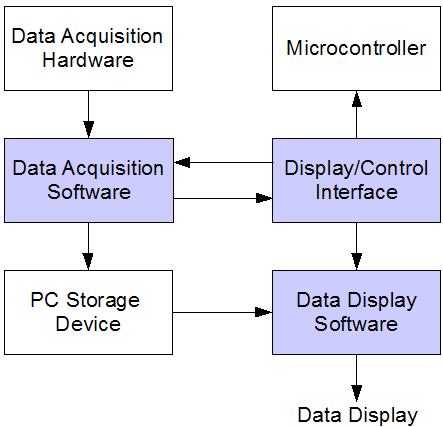
\includegraphics[scale=0.75]{../drawings/pcsoft_sub_diagram.png}
\end{center}
\caption[PC Software Block Diagram]{Block diagram of the PC Software Subsystem. White blocks
are not part of the subsystem.}
\label{fig:pcsoft sub diagram}
\end{figure}



\subsection[Design Decisions]{Design Decisions}
\subsubsection[Software Packages]{Software Packages}
There are two possible approaches to writing software that addresses both of 
these needs. The first is to utilize proprietary software development 
environments such as Matlab or Labview that bundle together data acquisition 
and Graphical User Interface (GUI) functionality in a relatively easy-to-use 
software package. The second is to manually build custom software to implement 
these functions.

The first approach considered was to use a proprietary signal processing 
environment. Perhaps the two most popular software packages in this area are 
Labview and Matlab. Labview is a development environment produced by National 
Instruments. Its base package offers user-friendly GUI development tools, ample 
drivers for data acquisition into the PC and even some signal processing 
functionality \cite{web:labviewbase}. Matlab is a widely-known computing 
environment for science and engineering applications with extensive signal 
processing functionality, GUI-development tools and a data acquisition toolbox 
for acquiring data into the PC \cite{web:matlab}. In other words, both packages 
offer exactly the needed functionality for this subsystem.

These features come at a price, however. The Labview base package costs 
\$1249 \cite{web:labviewbase}, while Matlab costs \$500 for a single-user license with an 
additional \$200 cost for the Data Acquisition Toolbox \cite{web:matlab}\cite{web:matlabdaq}. 
Furthermore, the nature of development environments like Labview and Matlab mean that 
developing a solution in either would result in a user interface that is only usable in 
Labview or Matlab. This means that end-users would be required to have working 
copies of whichever environment was used to develop the UI. Since home users and 
hobbyists are the target market for othe PC Diagnostics Tool, it is not reasonable 
to expect that every user will possess a copy of Matlab or Labview, and it is even less 
reasonable to assume that every user would purchase a copy in order to use the 
GUI. Building standalone applications in either environment is possible, but it 
comes at further cost: the Labview Application Builder for Windows, at \$999 \cite{web:labviewbase} 
or the Matlab Compiler, at \$500 \cite{web:matlabcompiler}. 

With these cost considerations in mind, a proprietary solution was ruled out. 
The next options explored were programming languages and software packages that 
were inexpensive or free and could be used to implement the PC software. It was 
first necessary to break down the two tasks of the subsystem to understand what 
was required. A break-down of necessary functionality required to implement each
 task is shown in Table \ref{tab:required functionality}.


\begin{table}[bhp]
\begin{tabular}{l | p{7cm}}
	Task & Necessary functionality \\ \hline
	Data acquisition and storage & Serial port communications library, File I/O \\ \hline
	Display/control interface & Serial port communications library, GUI library, 
	Signal/waveform plotting
\end{tabular}
\caption[Software functionality]{PC Software tasks broken down by the necessary 
functionality to perform each.}
\label{tab:required functionality}
\end{table}


Of the required functionality, nearly every modern programming language has a 
capacity for serial port communications, file I/O and building GUIs, so the deciding 
factor would lie elsewhere. Some deciding factors were brainstormed, and languages were 
evaluated based on cost, ease of implementation and whether or not the resulting 
software would work on different operating systems (i.e. whether it was ``cross-platform'').  
Programming languages considered were C++, Java, and Python. 

The language comparison performed is shown in Table \ref{tab:languages features}. 
Due to non-availability of concrete data, performance of all three languages was 
considered to be ``good-enough'' for the software's purposes. All three languages here are 
widely-used, and considering again the target market of hobbyists, it can be expected 
that the languages are optimized enough for the performance needed. In considering the 
ease of implementation for each language, it was found that all the languages had online 
documentation available as well as a serial port library. The only criteria on which they
differed was the ``level'' of the language. Programming languages can be classified by what 
level the code required to perform a given task is abstracted away from the low-level 
hardware details of accomplishing the task, with high-level languages being farther 
abstracted from the details \cite{web:suranathesis}. Higher level languages are therefore 
easier to implement code with because the language compile or interpreter handle things 
like memory management and CPU operations.


\begin{table}[bhp]
\begin{tabular}{l | c | p{6cm} | c}
	Language & Cost & Ease of implementation & Cross-platform? \\ 
	\hline
	C++ & Free & Online documentation, serial port library, medium-level language \cite{web:cpptut}\cite{web:cppserial} & No \\ 
	\hline
	Java & Free & Online documentation, serial port library, medium-level language \cite{web:javaapi}\cite{web:javaserial} & Yes \\
	\hline
	Python & Free & Online documentation, serial port library, high-level language \cite{web:pydoc}\cite{web:pyserial} & Yes \\
\end{tabular}
\caption[Language features]{Comparison of programming language features.}
\label{tab:languages features}
\end{table}


After careful consideration of each language's features, it was decided to use Python as 
the programming language. Choosing C++ has no obvious benefits while having the exclusive 
drawback of not being cross-platform, and while Java has, for the purposes of this subsystem, 
essentially the same features as Python, a Python implementation should be easier because of 
its status as a high-level programming language.

For the signal/waveform plotting, it was decided from the beginning that, given the target 
market of hobbyists, real-time data display would not be necessary. Furthermore, many 
hobbyists using the PC Diagnostics Tool will have some technical background in engineering, 
and perhaps even some experience with computation software like Matlab. It seems reasonable, 
then, to perform the data plotting in a numerical computational environment in order to 
allow users to easily extend whatever functionality is provided by the default PC software. 
GNU Octave, a free, open source, Matlab-like numerical computing software package, provides 
such an environment \cite{web:octave}.


\subsubsection[Software Implementation]{Software Implementation}
In order to facilitate the necessary software tasks outlined in Figure 
\ref{fig:pcsoft sub diagram}, some design options had to be sifted through. Specifically, 
how the data acquisition would be achieved. In order to prevent the act of data 
acquisition from tying up the resources of the user interface, it is necessary to launch 
the data acquisition software in a separate sub-process. This, however, introduces a 
problem of how the interface process and the data acquisition process will communicate with 
each other. There exist, however, several techniques that enable communication between 
processes, which are aptly called inter-process communication (IPC) techniques. Pipes are 
perhaps the simplest method among these, but it turns out that a necessary operating system 
call named \textit{fork()} does not work on Windows \cite{web:windowsfork}. Furthermore, 
after much testing, the Python workaround for this inconsistency was found to be non-functional. 
Sockets are the next-best choice because, while they are not the simplest method, sockets can
 communicate over a network. This opens up the possibility of the data acquisition software 
running on a separate machine from the interface, which could be useful for a few different 
applications.

There is another problem that the PC Software must solve: when using a Python application to 
implement the user interface and GNU Octave to perform data plotting, it becomes impossible to 
utilize IPC to enable communication between the two. Being that GNU Octave is open source, one 
solution is to use Octave's C++ headers and a software package called Simplified Wrapper and Interface
 Generator (SWIG) to directly call  GNU Octave's plot functions from the interface itself \cite{web:swig}. 
This turned out to not be feasible due to copyright issues: GNU Octave is distributed under the GNU 
GPL, a copyright license that requires any code that links to GPL'd code to itself be released under 
the GNU GPL \cite{web:gnugpl}. In the interests of potential future commercialization, it was desired 
that the code to the PC Software not become open source. A simple, effective solution to this is to 
use Python's \textit{subprocess} module to launch an instance of Octave that executes a data display 
script. Before the launch, data is written to a control file that the Octave script later reads 
to find out which data should be displayed. This enables on-demand data plotting without resorting 
to using GNU Octave headers.


\subsection[Software Listings \& Cost]{Software Listings \& Cost}

A list of software packages used for PC Software subsystem is shown in Table \ref{tab:software packages}. 
Python and GNU Octave have been previously discussed. PySerial is a cross-platform serial 
communications library for Python, and pywin32 is a Windows 32 API library for Python which is 
required for pySerial to work on Windows. All software packages are free and open source.


\begin{table}[h]
\begin{tabular}{l | p{8cm}}
	Software Package & Description \\ \hline
	Python & Programming language used to implement data acquisition and interface software. \\ 
	\hline
	pySerial & Serial port communications library for Python. \\
	\hline
	pywin32 & Windows 32 API library for Python, required for pySerial on Windows \\
	\hline
	\multicolumn{2}{l}{Total cost: \$0} \\
\end{tabular}
\caption[Software packages]{Software packages utilized by the PC Software subsytem, along with total cost.}
\label{tab:software packages}
\end{table}


\subsection[Software Design]{Software Design}
A block diagram of the PC software files is shown in Figure \ref{fig:pcsoft files diagram}. Blocks 
in blue represent files that execute code. Blocks in green are data/control files required for normal 
program operation. Blocks in red represent data that is saved to an end-user's PC storage device.
 A description of the functionality for each file in the software follows.


\begin{figure}[bhp]
\begin{center}
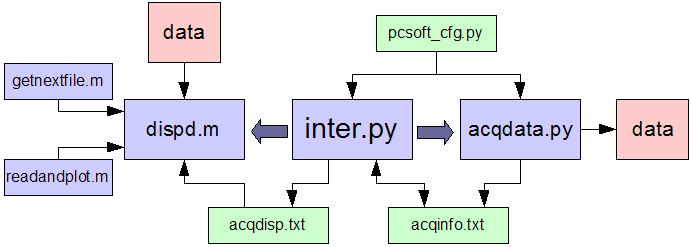
\includegraphics[scale=0.65]{../drawings/pcsoft_files_diagram.png}
\end{center}
\caption[PC Software Files Block Diagram]{Block diagram of the PC Software files. Blocks in blue
indicate files in which execution of code occurs. Blocks in green are data/control files. Blocks
in red represent acquired data.}
\label{fig:pcsoft files diagram}
\end{figure}


\subsubsection[inter.py]{inter.py}
This is the main hub of the PC Software subsystem. In addition to generating and displaying the 
main graphical front-end seen by the user, it performs the following tasks:

\begin{itemize}
\item Initiates the data acquisition process by launching the data acquisition software in a 
sub-process and communicating with it via sockets.
\item Enables user to specify configuration bits for the data acquisition hardware, including 
whether the input signal is analog or digital; allows user to enable/disable output.
\item Allows user to associate a mnemonic label with a data acquisition.
\item Provides to user a way to delete, scroll through and search previously saved data.
\item Enables on-demand data plotting by providing a method of displaying an acquisition; launches 
the GNU Octave data display script in a separate subprocess when such input has occurred.
\end{itemize}


A screenshot of the interface that inter.py creates is shown in Figure \ref{fig:pcsoft inter ss}. The
UI consists of three different areas: the Data Acquisition frame, the Data Display frame and the
Control Interface frame.

\begin{figure}[bhp]
\begin{center}
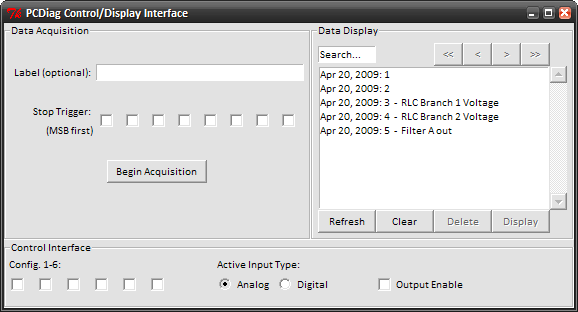
\includegraphics[scale=0.6]{../drawings/pcsoft_inter_ss.png}
\end{center}
\caption[PC Software Interface Screenshot]{Screenshot of the PC Software GUI front-end.}
\label{fig:pcsoft inter ss}
\end{figure}


The data acquisition process is initiated in the Data Acquisition frame by clicking on the 
``Begin Acquisition'' button. A series of checkboxes labeled ``Stop Trigger'' allows the user
 to define the bit pattern that the data acquisition software will detect to terminate the 
acquisition session. An optional label entry field allows the user to associate a label with 
an acquisition session as a means of organizing data that is captured by the software.


The Control Interface frame provides the user with configuration options for the acquisition
hardware. A group of 6 checkboxes labeled ``Config 1-6'' are general configuration options for
the currently active input. Two radio buttons provide control over the type of input signal,
and a last checkbox allows the user to enable or disable output.


The Data Display frame provides the user with an interface for managing previously acquired
data. The acquisition list displays and orders acquisitions by date and number. Labels are
displayed for acquisitions that have them. Because a user may eventually accumulate hundreds
of acquisitions, acquisitions are broken up into ``pages,'' which ensures that not too many
are displayed at one time. Four arrow buttons on the top right allow the user to go to the first 
page, the previous page, the next page or the last page. Four buttons at the bottom of the 
acquisition allow the user to perform various actions:

\begin{itemize}
\item ``Refresh'' - Refreshes the list.
\item ``Clear'' - Deletes every acquisition in the acquisition list.
\item ``Delete'' - Deletes only the selected acquisitions out of the list.
\item ``Display'' - Provides on-demand data plotting by launching the GNU Octave data display script.
\end{itemize}


\subsubsection[acqdata.py]{acqdata.py}
Acqdata.py is the data acquisition software. It is launched in a separate process when a user 
clicks on the ``Begin Acquisition'' button in the interface. This program quite simply reads
opens a connection with the serial port and reads data in continuously into a buffer until the 
stop trigger is detected. To avoid a possible buffer overflow, data is written to a binary file
when the buffer fills. In the case of large acquisitions, acqdata.py will break the acquisition 
output up into several parts. Output file names follow a format: \\

DDMonYYYY\_Np, \\

where ``DD'' is the two-digit date of the acquisition, ``Mon'' is a three letter abbreviation 
of the month of the acquisition, ``YYYY'' is the four-digit year of the acquisition, ``N'' is 
the number of the acquisition on the date it occurred and ``p'' is the letter of the acquisition part, starting with `a' and continuing through `z'. 


\subsubsection[pcsoft\_cfg.py]{pcsoft\_cfg.py}
This is a small configuration file for global variables that both inter.py and acqdata.py make
use of. This allows the user some degree of control over the operation of the software.


\subsubsection[acqinfo.txt]{acqinfo.txt}
This file is that stores information for every acquisition that the software processes. Each
acquisition is stored on a separate line with the following format: \\

DDMonYYYY\_N:[lp]{\tt\char'174}[label], \\

where ``DDMonYYYY\_N'' are the same as described for acqdata.py, where [lp] is either
the letter of the last part if the acquisition is multi-part or nothing if it is not, [label]
is the optional label associated with an acquisition, and `:' and `{\tt\char'174}' are separators used by
the software.


\subsubsection[acqdisp.txt]{acqdisp.txt}
A one-line text file that stores the name of the acquisition that should be displayed by
the GNU Octave data display script.


\subsubsection[dispd.m]{dispd.m}
Dispd.m is a script that runs in the GNU Octave environment. It reads acqdisp.txt to obtain
the name of the file it should plot, then reads in the binary data of the file and plots it.
Dispd.m uses getnextfile.m to obtain the next file part in the case of a multi-part
acquisition and readandplot.m to read in the binary acquisition data and display it.


\subsubsection[getnextfile.m]{getnextfile.m}
Called by dispd.m when the display file has multiple parts. Takes current filename and gets
the next file name to be displayed by incrementing the acquisition part letter by one.


\subsubsection[readandplot.m]{readandplot.m}
Called by dispd.m. Takes the current acquisition file name, reads in the data and plots it.
Sets the plot title as the date of the acquisition and, if the label exists, adds it to the
legend.



\subsection[Performance Data]{Performance Data}
Booga.


\subsection[Fault Analysis]{Fault Analysis}
Due to the nature of software, there is not a great deal that can go wrong with this subsystem 
because software does not degrade or fail randomly. However, an exhaustive look at the mechanisms and
operations invoked by the software reveal a few areas where damage to a user's PC may occur: file 
writing, socket communication and sub-process launching.

The program does do some file writing, but this is not troublesome in itself. In the event that the data
 acquisition process malfunctioned in some way, for instance the stop trigger that a user specified was 
never seen and the software simply continued to acquire data, the worst that would happen is the data
acquisition software would continue to write data until the user's storage device filled up, at which
point the process would error out and terminate due to not having any space left to write. The only way
this process could destroy a user's personal data is through some catastrophic failure of the PC storage
device and/or operating system. No software can be prepared for such a failure.

The socket communication itself does pose any trouble. If the user modified the program so that data
acquisition was performed on a separate machine and the interface communicated to the data acquisition
software over a network, it would open up the potential for another person to hijack the data acquisition
process. However, in such an event, the worst a hijacker could do would be to keep the data acquisition
process from terminating, which would again only fill up the storage device. Furthermore, this can only
occur if a user modifies the PC Software's default functionality. A user doing such a thing would certainly
understand the risks being taken.

Finally, subprocess launching is the last area where potential failure could occur. The user interface
launches subprocesses in two instances: when performing data acquisition and when displaying the plot
of selected data. The software contains code to re-launch subprocesses, so that a subprocess is launched
every time a data acquisition or display is triggered. The software contains code to \textit{wait()} 
for each subprocess before re-launching, which is important because \textit{wait()} is an operating system
call that suspends the operation of the current program until a child process has terminated. This in theory
should ensure that the program does not end up launching many subprocesses over the course of multiple 
acquisitions/displays. Assuming somehow that the \textit{wait()} call is ineffective, it may
be possible during normal use of the interface for a user to launch so many subprocesses that the user's
PC crashes, which could cause loss of unsaved data including acquisitions currently in process.

Luckily, even in such an event, considerable damage should not be possible. In the event that a large
number of subprocesses are inadvertently launched by a user, the user's PC should simply slowly grind
to a halt due to the number of resources the subprocesses are utilizing. This will probably result in
the computer freezing up, so the damage should cost at most however much unsaved data that was lost
during the crash costed. Since the target market of the PC Diagnostics Tool is home users and hobbyists,
there is little chance of valuable corporate data being lost here.


\subsection[Conclusions \& Recommendations]{Conclusions \& Recommendations}
Given that the PC Software subsystem has undergone no real-world testing, only 
simulation of input data using generated binary files, the subsystem needs further
testing. Currently the only untested portion of the subsystem is the data acquisition
over serial port, but having to handle real-world data may reveal mistakes in the
operation of the software that are, up to now, not understood.
